\section{Befehlssatzarchitektur}
\label{sec:befehlssatzarchitektur}

\begin{figure}[ht]
  \centering
  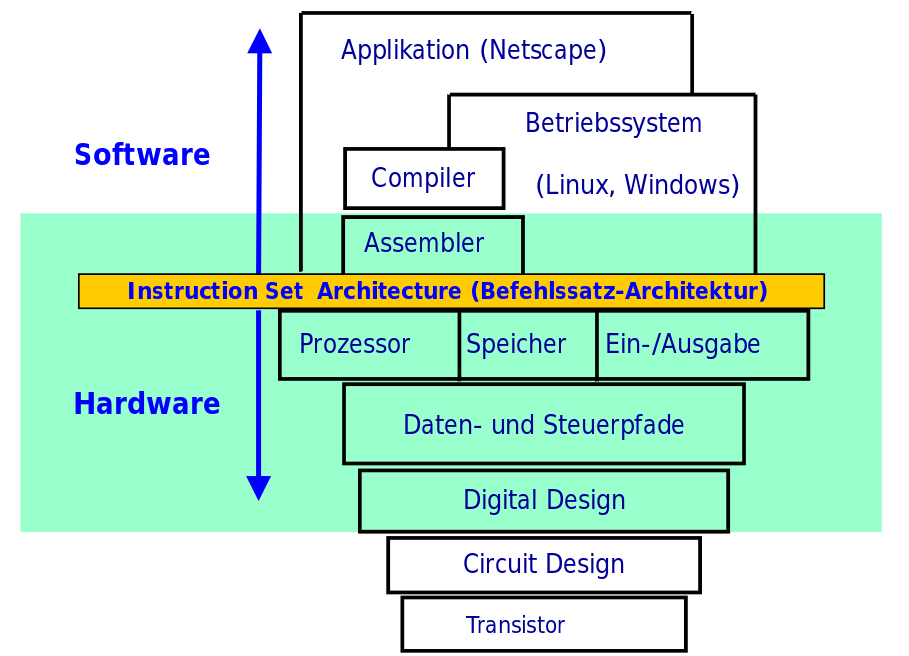
\includegraphics[width=0.33\textwidth]{ISA}
  \label{ISA}
\end{figure}

\textbf{ISA -- Aufgaben}
\begin{items}
	\item Wie werden Daten repräsentiert?
	\item Wo werden Daten gespeichert?
	\item Welche Operationen können auf den Daten ausgeführt werden?
	\item Wie werden die Befehle codiert?
	\item Wie wird auf die Daten zugegriffen?
	\item $\leadsto$ abstrahiert Hardware für den Maschinenprogrammierer
\end{items}

\textbf{Ausführungsmodelle}
\begin{figure}[ht]
  \centering
  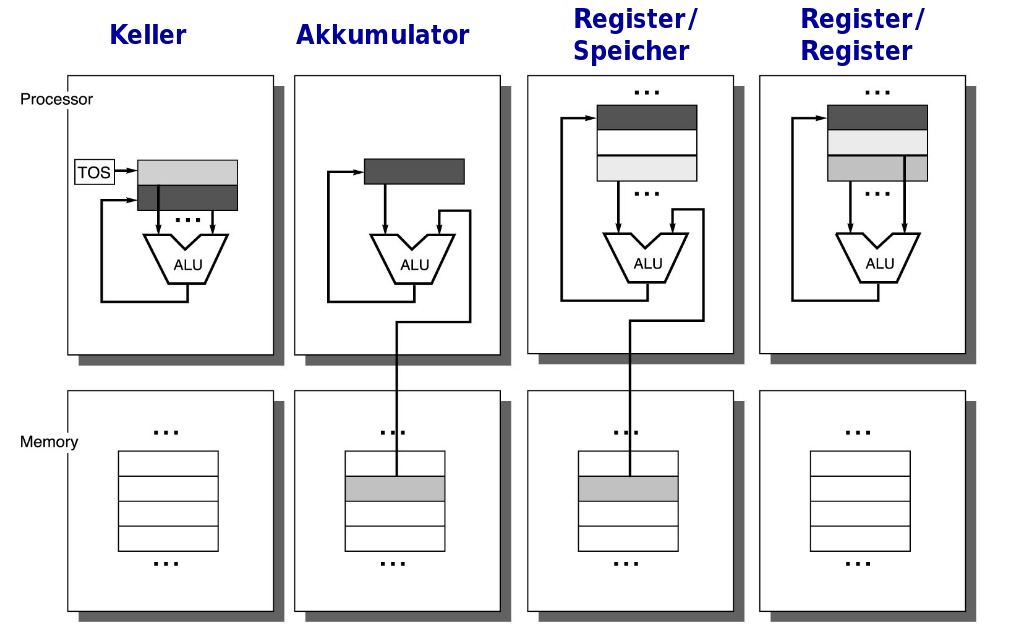
\includegraphics[width=0.33\textwidth]{Ausfuehrungsmodelle}
  \label{Ausfuehrungsmodelle}
\end{figure}

\textbf{Ausführungsmodell -- Register-Register}
\begin{items}
	\item Alle Operanden und Ergebnis stehen in Allzweckregistern
	\item \underline{Load/Store}: Bestimmte Befehle holen Operanden aus Hauptspeicher, schreiben Inhalte von Registern in Speicher
	\item \underline{Dreiadressformat}
	\begin{align*}
		\text{\code{load R2,A}} &\quad \text{\code{R2<-mem[A]}} \\
		\text{\code{load R3,B}} &\quad \text{\code{R3<-mem[B]}} \\
		\text{\code{add R1,R2,R3}} &\quad \text{\code{R1<-R2+R3}} \\
		\text{\code{store C,R1}} &\quad \text{\code{mem[C]<-R1}}
	\end{align*}
	\item \underline{Vorteile}: Einfaches und festes Befehlsformat, einfaches Code-Generierungsmodell, etwa gleiche Ausführungszeit der Befehle
	\item \underline{Nachteile}: Höhere Anzahl von Befehlen im Vergleich zu Architekturen mit Speicherreferenzen, längere Programme
\end{items}

\textbf{Ausführungsmodell -- Register-Speicher}
\begin{items}
	\item Ein Operand im Speicher, ein Operand im Register, Ergebnis in Speicher oder Register
	\item Explizite Adressierung mit/ohne Überdeckung
	\item \underline{Zweiadressformat}
	\begin{align*}
		\text{\code{add A,R1}} &\quad \text{\code{mem[A]<-mem[A]+R1}} \\
		\text{\code{add R1,A}} &\quad \text{\code{R1<-R1+mem[A]}}
	\end{align*}
	\item \underline{Vorteile}: Zugriff auf Daten ohne vorherige Ladeoperationen, Befehlsformat-Kodierung $\leadsto$ höhere Code-Dichte
	\item \underline{Nachteile}: Keine gleiche Operanden-Behandlung bei Überdeckungen, Taktzyklen pro Instruktion von Adressrechnung abhängig
\end{items}

\newpage

\textbf{Ausführungsmodell -- Akkumulator-Register}
\begin{items}
	\item \underline{Akkumulator}: Ausgezeichnetes Register, dient als Quelle eines Operanden und als Ziel für das Resultat (zweistellige Operationen)
	\item Implizite und überdeckte Adressierung
	\item Spezielle Befehle ermöglichen Operanden-Transport
	\item \underline{Einadressformat}
	\begin{align*}
		\text{\code{add A}} &\quad \text{\code{acc<-acc+mem[A]}} \\
		\text{\code{addx A}} &\quad \text{\code{acc<-acc+mem[A+x]}} \\
		\text{\code{add R1}} &\quad \text{\code{acc<-acc+R1}}
	\end{align*}
\end{items}

\textbf{Ausführungsmodell -- Keller}
\begin{items}
	\item Operanden einer zweistelligen Operation stehen auf den obersten zwei Kellerelementen
	\item Ergebnis wird auf Keller abgelegt
	\item Implizite Adressierung über Kellerzeiger (\code{tos})
	\item Überdeckung
	\item \underline{Nulladressformat}
	\begin{align*}
		\text{\code{add}} &\quad \text{\code{tos<-tos+next}}
	\end{align*}
\end{items}

\textbf{Ausführungsmodelle -- Übersicht} \\
\begin{items}
	\item 
	\begin{center}
		\code{C=A+B; D=C-B}
	\end{center}
	\begin{figure}[ht]
	  \centering
	  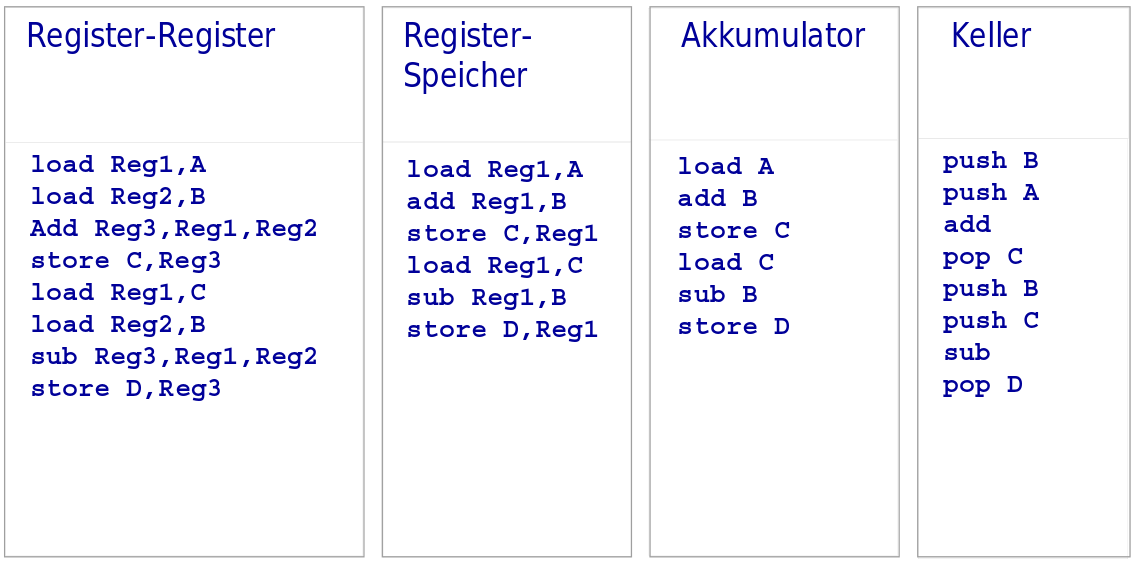
\includegraphics[width=0.33\textwidth]{UebersichtISA}
	  \label{UebersichtISA}
	\end{figure}
\end{items}